\documentclass[10pt,twoside]{article}
\usepackage[utf8]{inputenc}
\usepackage{amsmath}
\usepackage{amsfonts}
\usepackage{amssymb}
\usepackage[spanish,es-noshorthands]{babel}
\usepackage[T1]{fontenc}
\usepackage{lmodern}
\usepackage{graphicx,hyperref}
\usepackage{tikz,pgf}
\usepackage{multicol}
\usepackage{subfig}
\usepackage[papersize={5.5in,8.5in},left=.75cm,right=.75cm,top=1.5cm,bottom=1.25cm]{geometry}
\usepackage{fancyhdr}
\pagestyle{fancy}
\fancyhead[LE]{
\includegraphics[height=12pt]{Images/logo-colegio.png} Geometría $6^{\circ}$}
\fancyhead[RE]{}
\fancyhead[RO]{\textit{Germ\'an Avenda\~no Ram\'irez, Lic. U.D., M.Sc. U.N.}}
\fancyhead[LO]{}

\author{Germ\'{a}n Avenda\~no Ram\'{i}rez~\thanks{Lic. Mat. U.D., M.Sc. U.N.}}
\title{\begin{minipage}{.2\textwidth}

\includegraphics[height=1.75cm]{Images/logo-colegio.png}\end{minipage}
\begin{minipage}{.55\textwidth}
\begin{center}
Taller 1, Nociones básicas\\
Geometría $6^{\circ}$
\end{center}
\end{minipage}\hfill
\begin{minipage}{.2\textwidth}

\includegraphics[height=1.75cm]{Images/logo-sed.png} 
\end{minipage}}
\date{}
\begin{document}
\maketitle
Nombre: \hrulefill Curso: \underline{\hspace*{44pt}} Fecha: \underline{\hspace*{2.5cm}}\\

\section*{Lo que s\'{e}}
\subsection*{Recorre un cultivo hidrop\'{o}nico}
Para algunos productores de hortalizas, plantas medicinales, alimentos o plantas ornamentales, que no cuentan con terrenos apropiados o suelos libres de contaminación, los cultivos hidropónicos se han constituido en un método muy valioso que garantiza su derecho al trabajo. Además, su organización facilita las tareas de valoración y cuidado de las plantas, ya que todos se encuentran distribuídos en grupos de canales o tubos dispuestos en línea recta, permitiendo el paso de los encargados.

\begin{minipage}{0.25\textwidth}
Carmenza tiene un cultivo hidropónico de fresa. Para una exposición que quiere realizar frente a sus trabajadores, diseñó un dibujo para representar la forma en que está organizado. Observa el dibujo y responde.
\end{minipage}\hfill
\begin{minipage}{.75\textwidth}
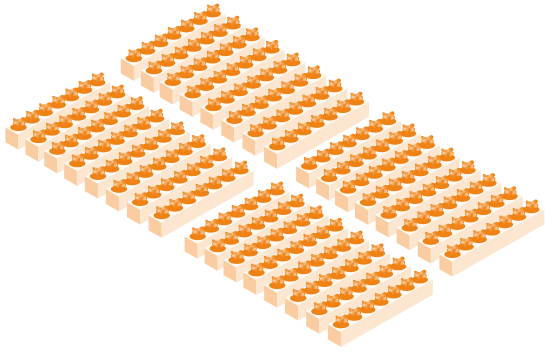
\includegraphics[scale=.45]{Images/CultivHidrop.png}
\end{minipage}
\begin{itemize}
\item Describe con palabras la manera como está organizado el cultivo hidropónico de Carmen.
\item ¿Qué crees que quizo representar con cada punto?
\item ¿Cuántos puntos hay en cada fila? ¿Y en cada columna?
\item Qué crees que se formaría si se unen los puntos de cada fila sin dejar espacio entre ellos?
\item ¿Y si se unen los puntos de cada columna?
\item Si quisiera encerrar cada una de las cuatro secciones que tiene el cultivo, ¿qué forma tendría la cerca?
\item Compara tus respuestas con dos de tus compañeros.
\end{itemize}
\section*{Aprendo algo nuevo}
El dibujo que elaboró Carmen para representar su cultivo muestra que se encuentra distribuido en cuatro secciones iguales y cada una de ellas está formada por plantas, representadas con puntos, alineados en filas y columnas.

Es fácil imaginar que el punto sea el elemento básico de cualquier dibujo por simple que parezca. De igual manera en geometría el elemento a partir del cual se definen otros, es el punto.

El \emph{punto} se define como un elemento geométrico que no está dotado de dimensión, es decir que no tiene longitud, ni ancho, ni alto. Solamente tienen posición. En adelante los puntos serán representados con una letra mayúscula.
\begin{itemize}
\item Volvamos a observar al menos una de las secciones que dibujó Carmen.

\begin{minipage}{.35\textwidth}
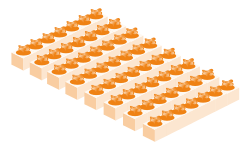
\includegraphics[scale=.45]{Images/CultivHidrop02.png} 
\end{minipage}\hfill
\begin{minipage}{.6\textwidth}
Cada 
\includegraphics[height=14pt]{Images/CultivHidrop03.png}  da la idea de punto pero matemáticamente no lo es, sin embargo nos permite imaginar el comportamiento de los elementos que se definen a partir del concepto de punto.
\end{minipage}
\item Si se dispusieran más puntos intermedios de tal manera que no quedaran espacios entre aquellos que conservan la misma dirección (que están en la misma fila o columna), tendríamos un ejemplo de lo que podría ser una recta.
\end{itemize}
\subsection*{Observa y responde:}
\tikz \filldraw[color=gray] (0,0) circle (4pt) (0.5,0) circle (4pt) (1,0) circle (4pt) (1.5,0) circle (4pt) (2,0) circle (4pt);\hspace*{2cm} \tikz \filldraw[color=gray] (0,0) circle (4pt) (0.2,0) circle (4pt) (0.4,0) circle (4pt) (0.6,0)circle (4pt) (0.8,0)circle (4pt);
\begin{itemize}
\item ¿Qué cambio se produce entre las imágenes?
\item ¿Cómo crees que se vería una imagen en la que los puntos estén cada véz más juntos?
\item ¿Se podría prolongar la cantidad de puntos infinitamente?
\item ¿Sabes cómo se llama en geometría el elemento que cumple esta condición? Una recta se puede entender como una sucesión indefinida de puntos que se prolongan en una misma dirección. La recta tiene una dimensión. Para nombrar la recta que pasa por los puntos A y B, se utiliza la notación: $\overleftrightarrow{AB}$
\end{itemize}
\begin{itemize}
\item Analiza la definición de recta que acabas de leer. Responde.
\item ¿A cuál dimensión crees que se refiere la definición de recta?
\item ¿Qué notación se utiliza para representar una recta que pase por los puntos $O$ y $P$? ¿Y por los puntos $C$ y $D$?
\end{itemize}
Piensa en el caso de que se conozca el punto de partida de una sucesión de puntos pero no el punto final.
\begin{itemize}
\item ¿Cómo representarías este nuevo elemento?
\item ¿Cuál sería su definición teniendo en cuenta la definición de recta que leíste anteriormente?
\item ¿Qué notación utilizarías para identificar un representante de este concepto?
\end{itemize}
La semirrecta es una porción de recta. En ella, se conoce el punto de origen pero no el final.
\subsubsection*{Aprendo algo nuevo otra vez}
\begin{itemize}
\item Piensa y responde. Copia la tabla y marca con una X las características que consideras que tiene una semirrecta. Ten en cuenta que es parte de una recta.
\end{itemize}
\begin{tabular}{|p{10cm}|l|l|}
\hline 
\textbf{Condición} & \textbf{Sí} & \textbf{No}\\ 
\hline 
Tiene una dimensi\'{o}n & & \\ 
\hline
Est\'{a} formada por una sucesi\'{o}n de puntos & & \\ 
\hline  
Se extiende infinitamente en dos sentidos por eso se representa con $\overleftrightarrow{AB}$ & &\rule[-0.3cm]{0cm}{0.8cm} \\ 
\hline 
Se extiende infinitamente en un solo sentido por eso se representa con $\overrightarrow{AB}$ & &\rule[-0.3cm]{0cm}{0.8cm}\\ 
\hline 
\end{tabular}

Otro concepto derivado del concepto de recta es el de segmento. En él aparte de
conocer el punto de origen se conoce el final. Por lo tanto, es un elemento que puede dotarse de medida ya que es finito. Para nombrar un segmento cuyos puntos de origen y final se denominan A y B se utiliza la notación $\overline{AB}$.
\subsection*{Ejercito lo aprendido}
\usetikzlibrary{arrows}
\definecolor{xdxdff}{rgb}{0.66,0.66,0.66}
\definecolor{qqqqff}{rgb}{0.33,0.33,0.33}
\begin{tikzpicture}[scale=.8,line cap=round,line join=round,>=triangle 45,x=1.0cm,y=1.0cm,>=stealth]
\clip(-3.26,-1.7) rectangle (6.44,4.32);
\draw [domain=-3.26:6.44,<->] plot(\x,{(--11.09--1.22*\x)/4.2});
\draw [domain=-3.26:6.44,<->] plot(\x,{(--5.46-0.72*\x)/2.88});
\draw [domain=-3.26:6.44,<->] plot(\x,{(--0.9-1.94*\x)/-1.32});
\draw [domain=-3.26:6.44,<->] plot(\x,{(-1.15-0.43*\x)/-3.36});
\begin{scriptsize}
\fill [color=qqqqff] (-1.38,2.24) circle (1.5pt);
\draw (-1.22,2.5) node {$A$};
\fill [color=qqqqff] (2.82,3.46) circle (1.5pt);
\draw (3.12,3.38) node {$B$};
\fill [color=qqqqff] (1.5,1.52) circle (1.5pt);
\draw (1.82,1.74) node {$C$};
\fill [color=xdxdff] (4.13,0.86) circle (1.5pt);
\draw (4.28,1.12) node {$D$};
\fill [color=xdxdff] (0.76,0.44) circle (1.5pt);
\draw (1,0.4) node {$E$};
\end{scriptsize}
\end{tikzpicture}
\begin{enumerate}
\item Nombra los puntos que estén en la misma recta.
\item ¿Qué elementos pasan o tienen como puntos incial o final a los puntos $C$ y $E$?
\subsection*{Evaluaci\'{o}n}
\begin{minipage}{.3\textwidth}
\usetikzlibrary{arrows}
\definecolor{xdxdff}{rgb}{0.66,0.66,0.66}
\definecolor{qqqqff}{rgb}{0.33,0.33,0.33}
\begin{tikzpicture}[scale=.8,line cap=round,line join=round,>=triangle 45,x=1.0cm,y=1.0cm]
\clip(-2.2,-1.06) rectangle (2.78,4.08);
\draw [domain=-2:2.78,<->] plot(\x,{(--0.5--0.66*\x)/0.64});
\begin{scriptsize}
\fill [color=qqqqff] (-0.92,-0.16) circle (1.5pt);
\draw[color=qqqqff] (-1.08,0.04) node {$M$};
\fill [color=qqqqff] (-0.28,0.5) circle (1.5pt);
\draw[color=qqqqff] (-0.58,0.5) node {$O$};
\fill [color=qqqqff] (1.19,2.01) circle (1.5pt);
\draw[color=qqqqff] (0.88,2.12) node {$N$};
\end{scriptsize}
\end{tikzpicture}
\end{minipage}\hfill
\begin{minipage}{.5\textwidth}
\item Realiza una lista de todas las semirrectas diferentes que se pueden trazar con punto inicial en: $M$, $N$ u $O$.
\item Escribe la notación correspondiente para cada elemento.
\begin{enumerate}
\item El segmento AB.
\item La recta que pasa por M y N.
\end{enumerate}	
\end{minipage}
\end{enumerate}
\end{document}
